%%%%%%%%%%%%%%%%%%%%%%%%%%%%%%%%%%%%%%%%%%%%%%%%%%%%%%%%%%%%%%%%%%%%%%%%
\chapter{Context}
%%%%%%%%%%%%%%%%%%%%%%%%%%%%%%%%%%%%%%%%%%%%%%%%%%%%%%%%%%%%%%%%%%%%%%%%

% \begin{center}
%   \begin{minipage}{0.5\textwidth}
%     \begin{small}
%       Hoofdstuk 2 besteedt aandacht aan de historie van de gesynthetiseerde stem en de hedendaags aanwezige technieken en initiatieven tot het realiseren van een menselijke stem met een eigen karakter. Het hoofdstuk wordt afgesloten met een afweging ten aanzien van de tegenwoordige initiatieven en de ontwikkelrichting van Prolody B.V.
%     \end{small}
%   \end{minipage}
%   \vspace{0.5cm}
% \end{center}

%%%%%%%%%%%%%%%%%%%%%%%%%%%%%%%%%%%%%%%%%%%%%%%%%%%%%%%%%%%%%%%%%%%%%%%%
\section{Inleiding}
%%%%%%%%%%%%%%%%%%%%%%%%%%%%%%%%%%%%%%%%%%%%%%%%%%%%%%%%%%%%%%%%%%%%%%%%

Spraak synthese is de kunstmatige reproductie van menselijke spraak. Computer systemen die voor dit doeleinde worden gebruikt, worden ook wel spraakcomputers, spraaksynthesizers of een text-to-speech (TTS) systeem genoemd. Deze systemen zijn ontwikkeld voor de translatie van zowel fonetische als natuurlijke taal naar een audio representatie. De kwaliteit van een spraaksynthese systeem wordt doorgaans geëvalueerd op basis van verstaanbaarheid en de similariteit met de menselijke stem. In dit hoofdstuk worden een aantal technieken uiteengezet voor het synthetiseren van menselijke spraak.

\begin{figure}[]
    \centering
    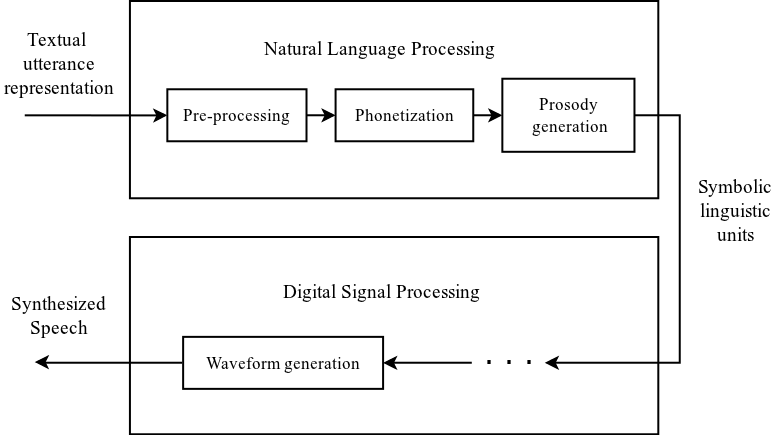
\includegraphics[width=0.5\textwidth]{figures/tts_system.png}
    \caption{Text-to-speech model \cite{speect}}
    \label{fig:tts}
\end{figure}

%%%%%%%%%%%%%%%%%%%%%%%%%%%%%%%%%%%%%%%%%%%%%%%%%%%%%%%%%%%%%%%%%%%%%%%%
\section{Probleemstelling}
%%%%%%%%%%%%%%%%%%%%%%%%%%%%%%%%%%%%%%%%%%%%%%%%%%%%%%%%%%%%%%%%%%%%%%%%

Vaak wordt gedacht dat het probleem van geschreven tekst vertalen naar spraak een probleem van 'omgekeerde spraakherkenning' is: huidige spraakherkenningssystemen worden als succesvol beschouwd als die opgenomen spraak kan vertalen naar de sequentie van woorden die zijn gezegd, dus men zou denken dat een TTS synthesizer begint bij de woorden in de tekst, die elk vertaalt naar een audio representatie, en de aparte resultaten aan elkaar hecht. Echter, het correct uitspreken van woorden is maar een onderdeel van spraak. Om een natuurlijke stem en een goede interpretatie van het gezegde te bewerkstelligen, moeten sommige woorden worden benadrukt en andere minder; een zin wordt op een betekenisvolle manier gefraseerd; er moet een gepaste contour van de $F_0$ (fundamentele) frequentie worden gekozen (de melodische contour in de stem), et cetera.

De moeilijkheid van de vertaalslag van tekst naar spraak, is het gebrek aan veel aspecten van informatie die van belang zijn voor spraak. Weliswaar representeert een zin alle woorden om de betekenis duidelijk te maken, maar het specificeert de frasering van een zin maar gedeeltelijk (door middel van bijvoorbeeld punctuatie), het specificeert niet de meer en minder benadrukte woorden en het geeft geen informatie over de intonatie of stemkwaliteit van een woord of frase.

TTS wordt vaak verdeeld in twee sub-problemen. Het eerste probleem adresseert de vertaling van tekst - een eigenlijk imperfecte representatie van taal zoals eerder aangegeven - in een linguïstieke vorm. Deze vorm bevat informatie over de fonemen die moeten worden geproduceerd, de duur en locaties van pauzeringen en de $F_0$ contour die moet worden gebruikt. Het tweede probleem adresseert de eigenlijke synthese van spraak. Het neemt de informatie uit het eerste probleem en vertaalt die naar een geluidsgolf.

Het eerste probleem, de tekst en linguïstieke analyse, wordt als volgt opgedeeld:
\begin{itemize}
    \item \textit{Tekst voorverwerking}: de detectie van het einde van de zin, tekst normalisatie (het volledig uitschrijven van nummers en afkortingen) en een grammaticale analyse, zoals het indelen van woorden in de bijbehorende, lexicale categorie (POS-tagging).
    \item \textit{Accentueren}: het aangeven van de nadruk die moet worden gelegd op bepaalde woorden.
    \item \textit{Uitspraak van woorden}: waarbij gelet wordt op de uitspraak van eigennamen, maar ook de desambiguatie van homoniemen \footnote{Een homoniem is een zelfstandig woord dat eenzelfde uitspraak heeft en tot eenzelfde woordsoort behoort, maar twee of meerdere geheel andere betekenissen heeft.}
    \item \textit{Fraseringen}: het fraseren van de zin door middel van intonatie.
    \item \textit{$F_0$ contour berekening}: waarbij een passende, melodische contour van de zin wordt berekend.
\end{itemize}

Het tweede probleem van spraak synthese wordt opgedeeld in twee delen:
\begin{itemize}
    \item de synthese van de spraak waveforms gegeven de gegenereerde, foneme delen in de eerste probleemstelling;
    \item de selectie en samenvoeging van zinsdelen gegeven de spraak waveforms.
\end{itemize}

%%%%%%%%%%%%%%%%%%%%%%%%%%%%%%%%%%%%%%%%%%%%%%%%%%%%%%%%%%%%%%%%%%%%%%%%
\section{Gesynthetiseerde stem}
%%%%%%%%%%%%%%%%%%%%%%%%%%%%%%%%%%%%%%%%%%%%%%%%%%%%%%%%%%%%%%%%%%%%%%%%

Text-to-speech synthese kent al een lange historie, beginnend bij Dudley's 'Voder' dat werd ontwikkeld bij Bell Laboratories en werd gedemonstreerd bij de World Fair in 1939 \cite{voder}. Een mens bestuurde de 10 bandpass filters van de 'Voder' om menselijke spraak te genereren. Pas vanaf de jaren '60 worden er systemen geïntroduceerd die automatisch spraak kunnen genereren op basis van linguïstieke representaties (zoals fonetische of tekstuele input). De twee belangrijkste technieken voor het synthetiseren van spraak waveforms zijn formantsynthese en concatinerende synthese (concatenative synthesis).

\subsection{Formantsynthese}
De eerste vorm van digitale spraaksynthese werd gerealiseerd met formantsynthese. Een formant is een smalle, piekende spectrale vorm die een oorsprong vindt in de resonantie van het menselijke spraakkanaal. Bij formantsynthese wordt gebruik gemaakt van additieve synthese en akoestieke modellering om spraak te genereren. Hierbij worden dus geen menselijke samples gebruikt.

\subsection{Concatenative synthesis}
Deze synthesetechniek synthetiseert geluid door middel van digitale, (korte) geluidssamples in een grote database slim te selecteren en samen te voegen (ook wel \textit{units} genoemd).

\subsubsection{Unit selection synthesis}
Een spraak synthesizer gebaseerd op concatenative synthesis gebruikt stukken natuurlijke spraak als bouwstenen om een arbritraire, nieuwe zin van spraak te reconstrueren \cite{nuance}. Een database van spraak \textit{units} is gemaakt met opnames van spraak. Door gebruik te maken van echte spraak worden een aantal karakteristieken van de stemacteur behouden. Een voordeel van \textit{Unit selection synthesis} is, dat wanneer er juiste \textit{units} worden gekozen, er een realistische stem met ook articulatie effecten ontstaat. Een ander voordeel is dat het een relatief eenvoudig systeem is, er hoeft weinig aandacht besteed te worden aan articulatie en synthese omdat er alleen gebruik wordt gemaakt van echte spraak \textit{units}.

In \textit{Unit selection synthesis} systemen wordt in een database gezocht naar foniemen die in dezelfde context als de \textit{target} foniemen voorkomen. Er wordt een \textit{penalty} voor het matchen van de gekozen foniem en de context gecaculeerd. Dit wordt gedaan door het verschil van de naburige foniemen in de \textit{target} en de naburige foniemen in de database te berekenen. De \textit{unit waveforms} van de \textit{target} worden daarna aan elkaar gezet (concatanation) door \textit{Pitch Synchronous Overlap and Add} (PSOLA) tussen aaneengesloten foniemen. Het algoritme past niet de prosodie aan, maar gebruikt dezelfde lengte, intonatie en articulatie van de foniem in de database. Het gebrek aan een goede, \textit{prosodic target} is een van de grootste tekortkomingen in dit systeem.

Om de ontwikkeling van een spraak \textit{unit} database te versnellen, zijn er automatische synthese \textit{unit} generation systemen ontwikkeld \cite{nakajima1994automatic}. Hierbij wordt de inventaris van spraak \textit{units} automatisch geannoteerd door middel van een al geannoteerde database (spraak waarvan de tekst al is getranscribeerd).


%%%%%%%%%%%%%%%%%%%%%%%%%%%%%%%%%%%%%%%%%%%%%%%%%%%%%%%%%%%%%%%%%%%%%%%%
\section{Hedendaagse technieken}
%%%%%%%%%%%%%%%%%%%%%%%%%%%%%%%%%%%%%%%%%%%%%%%%%%%%%%%%%%%%%%%%%%%%%%%%

\subsection{WaveNet}
WaveNet is een neuraal netwerk voor het genereren van audio waveforms \cite{45774}. Dit model is volledig probabilistisch en zelfvoorspellend, waarbij er een kansdistributie wordt berekend voor elk audio sample, geconditioneerd op alle vorige. Wanneer het wordt gebruikt in een tekst-to-speech toepassing, heeft het een state-of-the-art prestatie waarbij mensen het als significant beter en realistischer beoordelen dan de beste concatenative synthese systemen \footnote{\url{https://deepmind.com/blog/wavenet-generative-model-raw-audio}}. WaveNet kan ook worden gebruikt voor het herkennen van foniemen, voor bijvoorbeeld gebruik in concatenative synthesis.

WaveNet is ontwikkeld door DeepMind en ligt ten grondslag aan alle nieuwe text-to-speech systemen van Google die onder andere worden gebruikt in de Google Assistant \footnote{\url{https://cloud.google.com/text-to-speech/docs/wavenet}}.


\subsection{Tacotron}
WaveNet netwerken worden gemaakt met audio waveforms. Tacotron\cite{Wang2017TacotronTE} netwerken worden gemaakt met spectogrammen, een visuele representatie van het spectrum van frequenties van een signaal variërend over tijd. Het is een end-to-end generatief text-to-speech model dat direct spraak synthetiseert van karakters (letters). Gegeven \texttt{<tekst, audio>} paren wordt dit model volledig getraind, zonder gebruik te maken van een pre-trained netwerk. Het bereikt een \textit{naturalness score} van 3.82 van de 5 voor het Engels. Tacotron genereert spraak op een frame-niveau, wat significant sneller is dan modellen als WaveNet die genereren op sample-niveau. 

Omdat spectogrammen informatie verliezen over de positie van de fase in een frame, wordt het Griffin-Lim algoritme gebruikt om de audio waveforms te reconstruereren door de fase van de input spectogram te voorspellen. Het resultaat hiervan was enige fasevervorming in de resultaten. Tacotron is met 8 papers verbeterd tot Tacotron 2. In figuur \ref{fig:tacotron} wordt het eerste model van Tacotron weergegeven.

\begin{figure}[H]
    \centering
    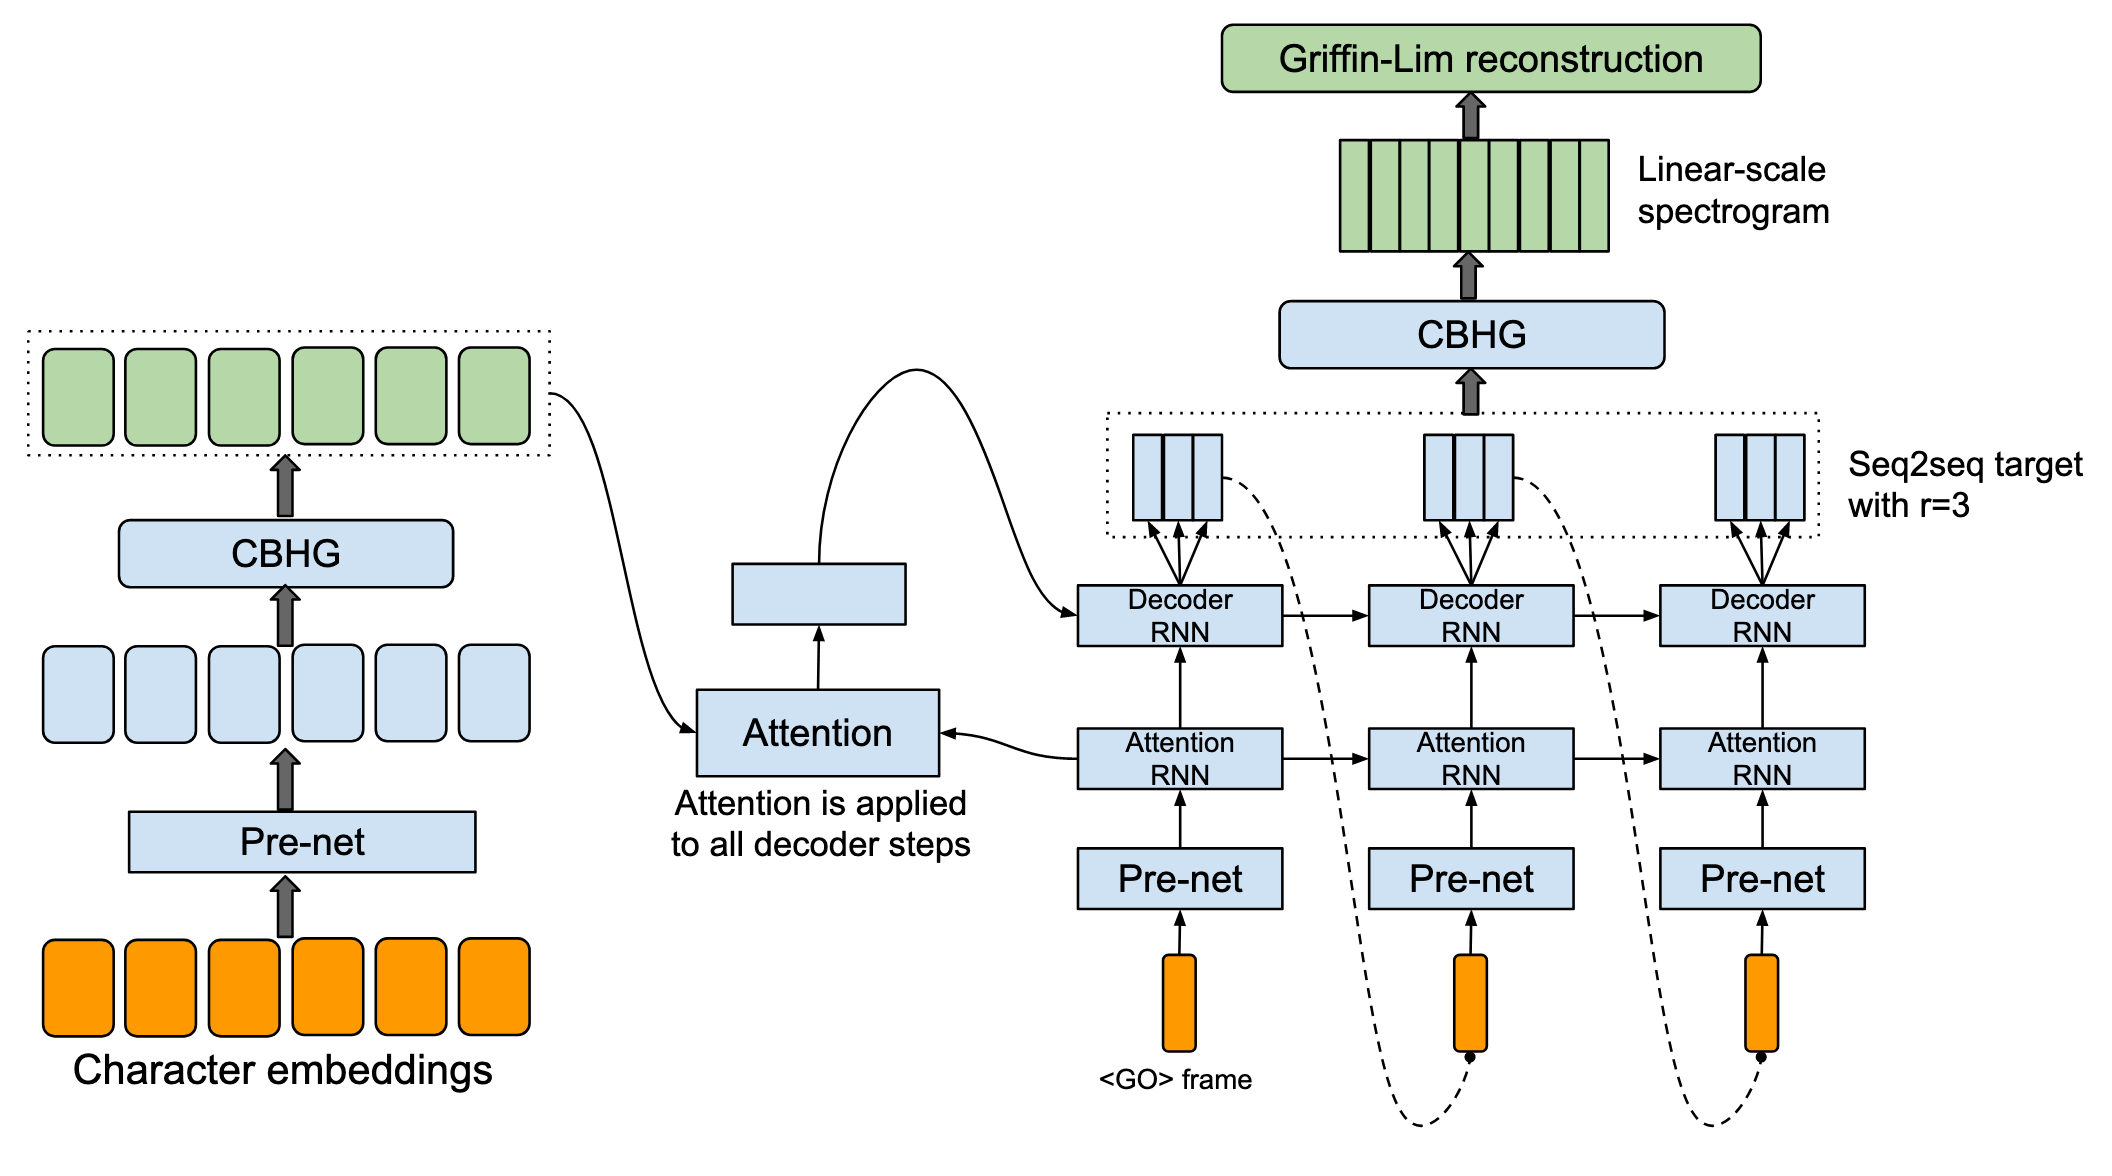
\includegraphics[width=\textwidth]{figures/tacotron.png}
    \caption{Model architectuur van Tacotron. Het model neemt karakters (letters) als input en geeft als output de corresponderende spectogram, wat daarna aan het Griffin-Lim reconstructie algoritme wordt gevoed om spraak te synthetiseren.}
    \label{fig:tacotron}
\end{figure}


\subsection{Deep Voice}
Deep Voice (3) is een volledig neuraal convolutie netwerk gebaseerd op attention\cite{Arik2017DeepVR}. Het neemt data van een \textit{multi-speaker} dataset, waarbij het netwerk traint op meerdere stemvarianten. De model architectuur van Deep Voice heeft drie componenten. Het heeft een volledige convolutie encoder, waarmee tekstuele kenmerken worden omgezet naar een interne, gevectoriseerde representatie. De decoder heeft tevens een volledige convolutie, waarmee de representaties die geleerd zijn door het netwerk via een attention mechanisme naar een audio representatie worden omgezet (mel-scale spectogrammen). De converter voorspelt de parameters voor de vocoder die wordt gebruikt voor het omzetten van de mel-scale spectrogrammen naar een audio signaal. Er is een Griffin-Lim vocoder, WORLD vocoder en een WaveNet vocoder. De model architectuur van Deep Voice 3 wordt weergegeven in figuur \ref{fig:deepvoice}. Ook is er een open-source implementatie van Deep Voice 3 \footnote{\url{https://r9y9.github.io/deepvoice3_pytorch/}}. 

\begin{figure}[H]
    \centering
    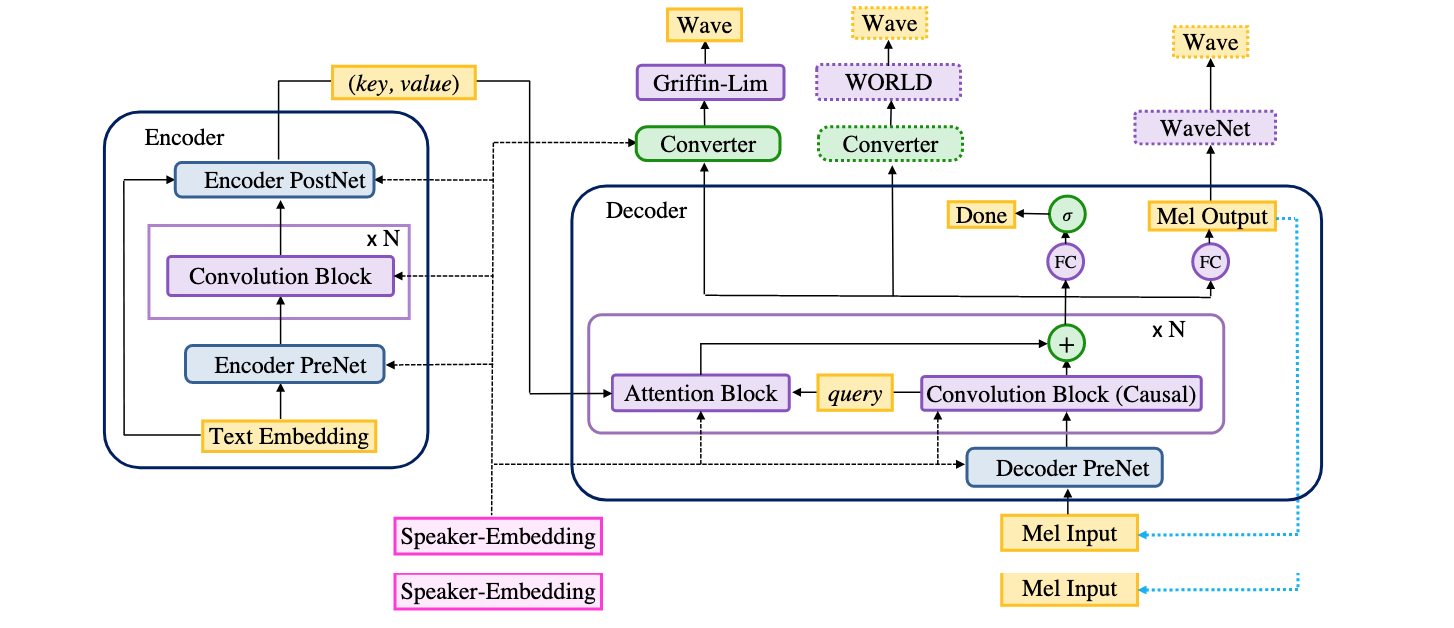
\includegraphics[width=\textwidth]{figures/deepvoice.png}
    \caption{Deep Voice 3 gebruikt convolutie lagen om tekst naar een \textit{key-value pair} representatie om te zetten in de Encoder module. De decoder leert en gebruikt deze representatie om die om te zetten naar mel-scale spectogrammen dat corresponderen met de output audio waveform. De zogenaamde \textit{hidden states}, de latente lagen in het neurale netwerk, worden dan aan de converter module die voorspellingen maken over de vocoder parameters voor het synthetiseren van de audio waveform.}
    \label{fig:deepvoice}
\end{figure}

\subsection{Char2Wav}
Char2Wav is een end-to-end neural netwerk model voor spraak synthese\cite{sotelo2017char2wav}. Dit netwerk heeft twee componenten: een \textit{reader} en een neurale vocoder. De \textit{reader} is een encoder-decoder model met een attention module. De encoder is een bidirectioneel, recurrent neuraal netwerk dat tekst of foniemen als input neemt. De decoder is ook een neuraal netwerk met de attentie module dat akoestieke features maakt voor de vocoder. De neurale vocoder is een SampleRNN, waarmee audio waveforms worden gegenereerd gegeven de features van de decoder. Char2Wav leert audio waveforms te produceren door tekst, zonder dat daar een translatie tussen komt zoals spectogrammen. Een aantal voorbeelden zijn te vinden op de website van het onderzoek \footnote{\url{http://josesotelo.com/speechsynthesis/}}.

\subsection{Parrotron}
Parrotron is een end-to-end speech-to-speech neuraal netwerk dat een input van een spectogram direct naar een ander spectogram kan converteren, zonder dat daar een intermediaire representatie tussen zit\cite{biadsy2019parrotron}. Het netwerk heeft een encoder module, een spectogram en foniemen decoder en een vocoder om de audio waveform the synthetiseren. Het netwerk demonstreert dat het, gegeven een stem met een accent, een bepaalde prosodie en achtergrond ruis, het om kan zetten naar een \textit{target} speaker met een specifiek accent, prosodie en consistente articulatie. In het onderzoek wordt het gebruikt om niet-verstaanbare spraak of spraak met een accent te normaliseren, maar er wordt gehypothetiseerd dat dit ook andersom werkt. Een aantal voorbeelden zijn te vinden op de website van het onderzoek \footnote{\url{https://google.github.io/tacotron/publications/parrotron/index.html}}.






\subsection{Tacotron 2}
Tacotron 2 is een verbeterde versie van Tacotron, waarbij onder andere een WaveNet vocoder wordt geïntroduceerd\cite{Shen2018NaturalTS}. In plaats van $F_0$ features, linguistieke en andere features worden mel-scale spectograms gebruikt als input naar de WaveNet vocoder. Een zeer goede, open-source, licentievrije implementatie is ontworpen door NVIDIA en kan worden gebruikt om nieuwe stemvarianten te ontwikkelen \footnote{\url{https://github.com/NVIDIA/tacotron2}}. Deze implementatie gebruikt WaveGlow als vocoder.




\subsubsection{Prosody Embedding}
In een recent onderzoek wordt Prosody Embedding geïntroduceerd\cite{skerry2018towards}. Er wordt gebruik gemaakt van `global style tokens' (GSTs) die simultaan worden getraind binnen het netwerk van Tacotron. Deze embeddings worden getraind zonder expliciete labels, wat betekent dat er geen expliciete categorieën worden hoeven aangegeven per spraakfragment, maar modelleren desondanks veel expressie in spraak. Deze embeddings kunnen ook gestuurd worden, onafhankelijk van de tekstuele input. Er is een onofficiële open-source implementatie met een aantal voorbeelden \footnote{\url{https://syang1993.github.io/gst-tacotron/}}.

Ook zijn op de website van het onderzoek een aantal voorbeelden te vinden \footnote{\url{https://ai.googleblog.com/2018/03/expressive-speech-synthesis-with.html}}.

\begin{figure}[H]
    \centering
    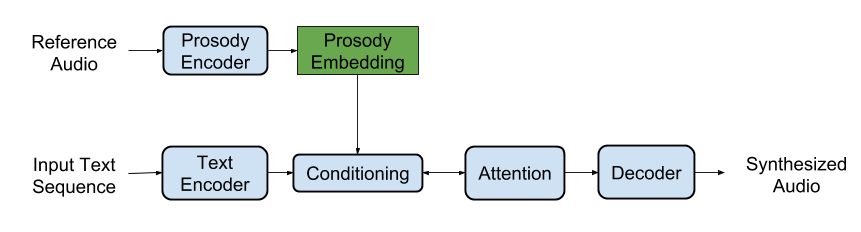
\includegraphics[width=0.75\textwidth]{figures/tacotron_prosody.png}
    \caption{Model architectuur van `Towards End-to-End Prosody Transfer for Expressive Speech Synthesis with Tacotron' \cite{skerry2018towards}}
    \label{fig:tts}
\end{figure}

\subsection{WaveGlow}
WaveGlow is een op flow-gebaseerd netwerk dat spraak van hoge kwaliteit kan genereren van mel-spectogrammen. WaveGlow komt voort uit WaveNet en Glow (een generatief model) \footnote{\url{https://openai.com/blog/glow/}} en kan, zonder gebruik te maken van het sterke maar langzame, zelfvoorspellende vermogen van WaveNet, zeer realistische audio waveforms synthetiseren \footnote{\url{https://nv-adlr.github.io/WaveGlow}}

%%%%%%%%%%%%%%%%%%%%%%%%%%%%%%%%%%%%%%%%%%%%%%%%%%%%%%%%%%%%%%%%%%%%%%%%

%%%%%%%%%%%%%%%%%%%%%%%%%%%%%%%%%%%%%%%%%%%%%%%%%%%%%%%%%%%%%%%%%%%%%%%%
\subsection{Sample Efficient Adaptive Text-to-Speech}
Sample Efficient Adaptive Text-to-Speech bouwt voort op een \textit{multi-speaker model}, gebruikmakend van WaveNet, en leert onafhankelijk de latente \textit{embedding} van elke spreker\cite{chen2018sample}. Latente embeddings zijn een set van vectoren of reële getallen die een netwerk leert om een set informatie om te zetten in een andere set informatie, bijvoorbeeld het vertalen van een tekst naar een mel-spectogram. Het doel van dit netwerk is niet het leren van de \textit{weights} dat een text-to-speech systeem goed maakt, maar het produceren van een netwerk dat weinig data nodig heeft en snel kan aanpassen aan nieuwe stemvarianten. Gegeven een al goed getraind text-to-speech netwerk, zoals een WaveNet of Tacotron (2) netwerk met veel spraakdata en de juiste hyperparameters, kan het met weinig data van een andere stem zeer effectief een andere stemvariant leren, gebaseerd op een combinatie van de originele stem en de \textit{input} stem. Met maar een aantal minuten aan spraakdata van een nieuwe spreker, kan het model met deze nieuwe \textit{speaker embedding} een zeer realistische en natuurlijke stem genereren.

Dit onderzoek biedt dus de mogelijk om, gegeven een al goed getraind text-to-speech model, op een snelle, effectieve manier meerdere stemvarianten te genereren. Hiervoor is slechts een aantal minuten spraakdata nodig van de te emuleren spreker, zoals een met een accent. Dit is voordeliger dan het volledig opnieuw trainen van een netwerk op een nieuwe stem, gezien het volledig nieuw trainen van een stem veel spraakdata en tijd vergt, en de juiste parameters voor het netwerk moeten zijn gekozen.

Een aantal audio fragmenten zijn beschikbaar gesteld op de website van het onderzoek 
\footnote{\url{https://sample-efficient-adaptive-tts.github.io/demo/}}.


%%%%%%%%%%%%%%%%%%%%%%%%%%%%%%%%%%%%%%%%%%%%%%%%%%%%%%%%%%%%%%%%%%%%%%%%
\section{Afweging en advies}
%%%%%%%%%%%%%%%%%%%%%%%%%%%%%%%%%%%%%%%%%%%%%%%%%%%%%%%%%%%%%%%%%%%%%%%%
Gegeven de recente publicatiedatum, de in productieomgevingen geteste architectuur en vooral adequate, open-source en licentievrije implementatie wordt aangeraden Tacotron 2 met WaveGlow te gebruiken als neuraal netwerk model om een Nederlands gesynthetiseerde stem te creëren (de \textit{baseline}). Het geeft tevens veel controle over de te genereren stem, omdat het goed werkt als \textit{single-speaker} model, in contrast met Deep Voice 3 dat een \textit{multi-speaker} model gebruikt. Nadat het netwerk is getraind, kan worden gekeken naar het trainen van `global style tokens' voor het genereren van meer expressieve spraak, hoewel een officiële implementatie nog ontbreekt. Ook kunnen meerdere stemvarianten op een relatief eenvoudige wijze ontwikkeld met SEATS, nadat de `weights' van het netwerk van de \textit{baseline} stem zijn getraind.